\section{problem 3}
\textit{Let a signal and interpolation kernel be given by}
\[
x[n] = \begin{cases}
   2, & n = 0\\
   1, & n = 1\\
   0, & \text{elsewhere} 
\end{cases}
\]
\[
g[n] = \begin{cases}
    -1, & n = -1\\
    3, & n = 0\\
    -1, & n = 1\\
    0, & \text{elsewhere}
\end{cases}
\]
\subsection{1.}
\textit{Upsample $x[n]$ by a factor 3 and sketch the upsampled signal.}
Here we upsample the signal by inserting two zeroes between every original sample.
There the first sample is 2 and the second is 1, we then insert two zeroes in between.
\[x[n] = [2,1,0,0] \Rightarrow [2,0,0,1,0,0,0,0,0,0,0,0]\]

\begin{figure}[!htb]
    \centering
    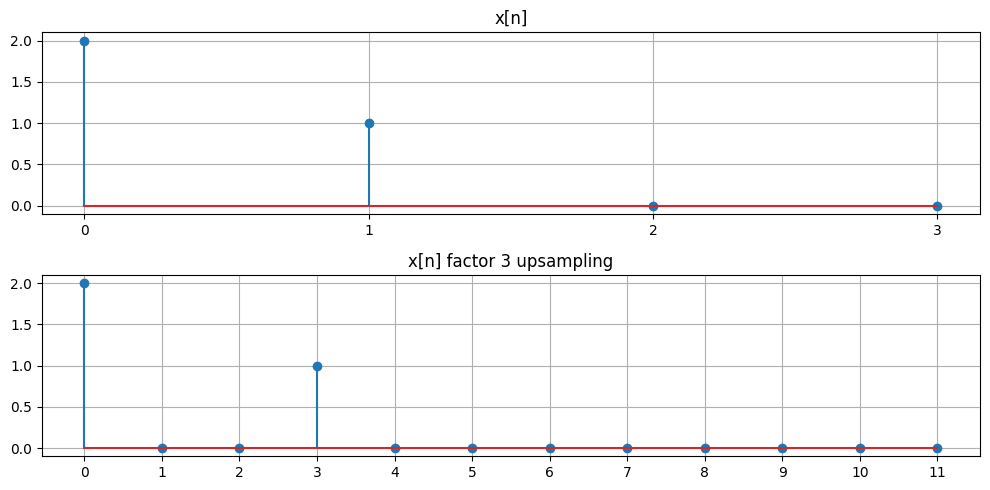
\includegraphics[width=0.7\textwidth]{p3_upsampling.png}
\end{figure}

\subsection{2.}
\textit{Compute the interpolated values $x_1[1]$ and $x_1[2]$ using first linear interpolation and 
second the proposed $g[n]$ kernel.}
To implement the linear interpolation scheme, we use the formula for the general interpolation:
\[x_{I}[n] = \sum_{m=-\infty}^{\infty}x[m]g_r[n-mI]\] %each original sample x[m] places a shifted scaled copy of the kernel at n = mI
In our case we only have $x[0] = 2$ and $x[1] = 1$, so only m = 0 and 1 contributes.
And uses the kernel 
\[
g_{lin} = \begin{cases}
    1 - \frac{|n|}{l}, & -l < n < l\\
    0, & \text{otherwise}
\end{cases}\]
%side 716 i bogen og 722
Substituing this into the interpolation formula:
\[x_{I}[n] = 2g_r[n] + 1 \cdot g_r[n-3]\]
The ideal interpolation is from negative to positive infinity, however this is impractical and impossible.
The practical approach is to only do it from all the original samples x[m], left and right of the current sample.
Thus when we build our linear interpretation keral from the cases above, we have to extend the range in both directions.
Our kernel values become:
\[g_{lin}[0] = 1, 
\qquad
g_{lin}[\pm1] = 1 -\frac{1}{3} = \frac{2}{3},
\qquad
g_{lin}[\pm2] = 1 -\frac{2}{3} = \frac{1}{3},
\qquad
g_{lin}[\pm3] = 0\]
leading to:
\[
\begin{array}{c|ccccccc}
n &-3&-2&-1&0&1&2&3 \\ \hline
g_{lin}[n] &0&\frac{1}{3}&\frac{2}{3}&1&\frac{2}{3}&\frac{1}{3}& 0
\end{array}
\]
Our original sequence was x[n], and when linearly interpolated, becomes:
\[
x_I[0] = 2,
\qquad
x_I[1] = \frac{5}{3},
\qquad
x_I[2] = \frac{4}{3},
\qquad
x_I[3] = 1
\qquad
x_I[4] = \frac{2}{3},
\qquad
x_I[5] = \frac{1}{3},
\qquad
x_I[6] = 0
\]
\begin{figure}[!htb]
    \centering
    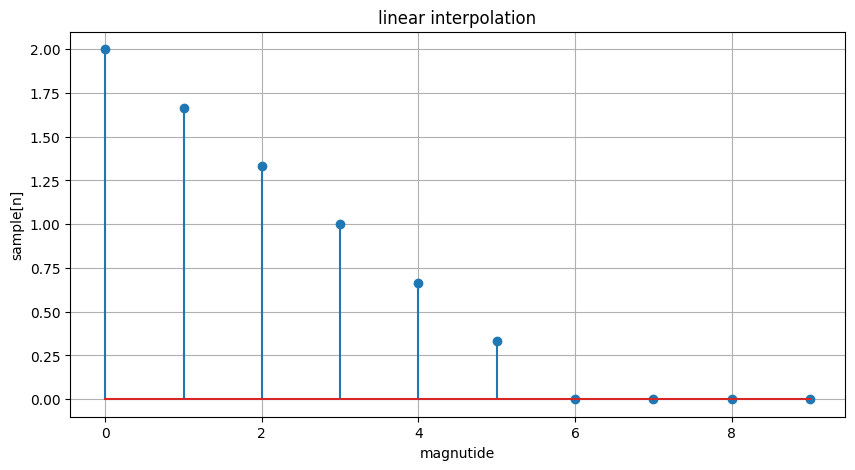
\includegraphics[width=0.7\textwidth]{p3_linear.png}
\end{figure}

As for the propsed interpolation kernel $g[n] \Rightarrow g_p[n]$, renamed for convienience.
Starting from the same interpolation formula:
\[x_p[n] = 2g_p[n]+g_p[n-3]\]

\[
x_p[-1] = 2g_p[-1]+g_p[(-1)-3] = 2(-1)+0 = -2 ,
\qquad
x_p[0] = 2g_p[0]+g_p[0-3] = 2(3) + 0 = 6,
\qquad
x_p[1] = 2g_p[1]+g_p[1-3] = 2(-1)+0 = -2,
\qquad
\]

\[
x_p[2] = 2g_p[2]+g_p[2-3] = 2(0) + (-1) = -1,
\qquad
x_p[3] = 2g_p[3]+g_p[3-3] = 2(0) + 3 = 5,
\qquad
x_p[4] = 2g_p[4]+g_p[4-3] = 2(0) + (-1) = -1,
\]
\[
\qquad
x_p[5] = 2g_p[5]+g_p[5-3] = 0 + 0 = 0 ,
\qquad
\]

leading to:
\[
x_I[-1] = -2,
\qquad
x_I[0] = 6,
\qquad
x_I[1] = -2,
\qquad
x_I[2] = -1,
\qquad
x_I[3] = 5,
\qquad
x_I[4] = -1,
\qquad
x_I[5] = 0,
\]
\begin{figure}[!htb]
    \centering
    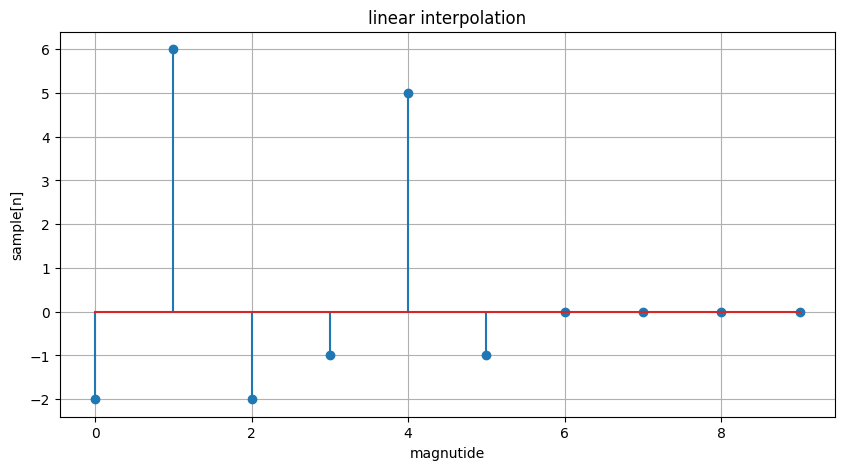
\includegraphics[width=0.7\textwidth]{p3_proposed_inter.png}
\end{figure}
\subsection{3.}


% \[
% \delta[l] = \begin{cases}
%     \sigma^2, & \text{if } l = 0\\
%     0, & \text{if } l \neq 0
% \end{cases}
% \]